\scanpage{22}

\deleted{M. DUFOUR\\
VARITYPISTE\\
131, RUE LECOURBE\\
PARIS XV$^{\mathrm e}$\\
\figure{\begin{tikzpicture}\fill (0,0) rectangle (.12,.12);\end{tikzpicture}}\\
C. C. P. Paris 14.143-34\\
R. M. 140.029}
\figure{\begin{tikzpicture}\draw (0,1.6)--(.7,0);\draw (1.1,1.5)--(1.7,.65);\draw (1.8,1.5)--(1.95,1.05);\end{tikzpicture}}

$A$ algèbre \inserted{locale noeth. complète,}
f$^t$ simple sur $k$ pour sa
topologie habituelle, alors $A$
est-il f$^t$ simple sur $\unsure{K|k}$ pour sa
topologie discrète ???.
\figure{\begin{tikzpicture}\draw (0,0)--(0,.5) to[out=90,in=180] (.2,.7)--(2.6,.7) to[out=0,in=10] (2.55,.8);\end{tikzpicture}}

\deleted{1°) Cas $p>0$}
On se \unsure{ramènera|ramène} au cas où $k$ est le
corps premier (plus gén. un corps \uline{parfait})
\inserted{\unsure{ou même} où $K/k$ est séparable, $K$ \unsure{le c. résiduel}}

\deleted{\unsure{1°)} \uline{Cas $\unsure{p>0|p=0}$}}
\unsure{Alors on a.}
$A\simeq K[[t_1,\ldots,t_n]]$, $K/k$
une extension \uline{séparable}.
\deleted{$\unsure{K}$ est form$^t$ simple sur
$k$, il suffira que $A$ le soit sur $K$.}
\deleted{$\unsure{K}$}

\unsure{1°)} \uline{Cas $p>0$}

Supposons que $K/k$ a une $p$-base
\uline{finie}, i.e.
\margin{$\Omega_{K/k}$ est fini sur $K$.}

\deleted{Si $K$ est parfait, alors}
\deleted{Alors $A$ est un anneau}

\deleted{$A$, ayant une $p$-base \inserted{$(t_1,\ldots,t_n)$},
sur $K$, est f$^t$ simple sur $K$.}
\deleted{\unsure{ayant une $p$-base},}
\deleted{\unsure{Il suffit} de connaître une
$p$-base de $A$ sur $k$. Il en existe si
$K$ est fini sur $K^p$, on prend une $p$-base
$(x_1\unsure{\text{--}|,}\,x_{\unsure{m|n}})$ de $K$, et y adjoint $t_1,\ldots,t_n$.}
\figure{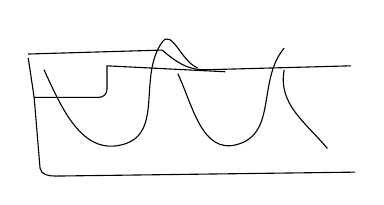
\begin{tikzpicture}[x=.5cm,y=.5cm]
\draw (0,3.1)--(3.4,3.2) to[out=-40,in=180] (4.5,2.7)--(8.2,2.8);
\draw (0,3)--(.15,2)--(1.8,2) to[out=0,in=-90] (2,2.2)--(2,2.8)--(5,2.65);
\draw (.4,2.7) to[out=-65,in=195] (2.4,.8) to[out=15,in=-125] (3.4,3.4) to[out=55,in=160] (4.3,2.75);
\draw (3.8,2.6) to[out=-65,in=195] (5.3,.8) to[out=15,in=-130] (6.5,3.25);
\draw (6.5,2.7) to[out=-100,in=130] (7.6,.7);
\draw (.15,2)--(.3,.2) to[out=-80,in=180] (.7,0)--(8.3,.1);
\end{tikzpicture}}

En la complétant par les $t_i$, on trouve
une $p$-base de $A$ sur $k$, et $K(A^p)=K\otimes_{K^p}A^p$.
[cf ``\unsure{Diff.}'']. Donc dans ce cas \unsure{on gagne}.

\mspage{21}
